\chapter{Fundamentação teórica e revisão bibliográfica}\label{cap2-revisao-bibliografica}

Este capítulo apresenta conceitos teóricos e a bibliografia utilizada
para contextualizar o problema estudado e as escolhas metodológicas
adotadas. São discutidos o Problema do Caixeiro Viajante (TSP) no
contexto da otimização combinatória
\autocite{cook2012pursuit,rosenkrantz1977analysis}, sua importância
geral e exemplos de utilização. Também são apresentadas generalizações
do problema e sua relação com problemas de roteamento de veículos e
variantes correlatas
\autocite{raff1983routing,bodin1981state,tan2021vehicle}, heurísticas e
meta-heurísticas clássicas para o TSP
\autocite{croes1958method,lin1973efficient,voudouris1999tsp},
aprofundando-se então no tópico de algoritmos genéticos e algoritmos
meméticos \autocite{larranaga1999genetic,goldberg1989genetic},
princípios de computação em GPU
\autocite{nvidia2024cuda,schulz2013gpu,tsp_gpu}, taxonomias de
paralelização de meta-heurísticas
\autocite{crainic2003parallel,crainic2010parallel,alba2005parallel} e de
comparação estatística de algoritmos de otimização
\autocite{demsar2006statistical}.

\section{Otimização combinatória e o Problema do Caixeiro Viajante}\label{sec-21-otimizacao-tsp}

O TSP pode ser formulado, na versão simétrica\footnote{Na versão
  assimétrica do TSP, os custos de viagem entre pares de cidades podem
  diferir dependendo da direção (ou seja, \(c_{ij} \neq c_{ji}\)). Em
  TSPs simétricos, o custo do cálculo de distâncias pode ser
  representado por uma matriz triangular que armazena apenas uma das
  metades (superior ou inferior) sem a diagonal, o que reduz o número de
  entradas únicas de \(n^2\) para \(n(n-1)/2\).}, como um problema de
encontrar um ciclo hamiltoniano de custo mínimo --- podendo este ser a
distância percorrida, combustível gasto, ou mesmo uma combinação de
fatores. Para fins deste trabalho, o custo será também chamado de
distância --- em um grafo completo não direcionado \(G = (V, E)\), no
qual cada vértice em \(V\) representa uma cidade e cada aresta
\((i, j) \in E\) possui um custo \(c_{ij} \geq 0\) entre as cidades
\(i\) e \(j\) \autocite{cook2012pursuit}. O objetivo é determinar uma
combinação das cidades que minimize a soma total dos custos, retornando
à cidade de origem. Geralmente em aplicações práticas assume-se que a
matriz de custos é métrica e euclidiana, isto é, os custos derivam de
distâncias euclidianas entre coordenadas no plano.

Do ponto de vista da complexidade, o TSP é um problema NP-difícil em sua
forma de otimização e NP-completo em sua forma de decisão
\autocite{cook2012pursuit}. Isso significa que, em geral, não se conhece
um algoritmo em tempo polinomial que resolva instâncias arbitrárias em
grande escala. Mesmo que seja relativamente fácil verificar o custo de
uma ou várias soluções candidatas, não podemos afirmar que esta é a
solução exata em tempo polinomial. Algoritmos exatos clássicos e
modernos expõem limites distintos. O algoritmo \texttt{Held-Karp}
\autocite{held1962dynamic} reduz a enumeração direta de tours de
\(O(n!)\) para tempo \(O(n^2 2^n)\), mas exige espaço \(O(n 2^n)\). Por
isso, apesar de ser assintoticamente superior à força bruta, sua tabela
de programação dinâmica cresce exponencialmente em memória e o torna
impraticável para instâncias moderadas. Já o \texttt{Concorde}
\autocite{cook2012pursuit} segue outra família
metodológica: combina relaxações de programação linear inteira, planos
de corte e ramificação (\emph{branch-and-cut}). Ele não possui o limite
\(O(n^2 2^n)\) do Held-Karp; no pior caso, continua sujeito ao
crescimento exponencial inerente ao TSP exato, mas na prática resolve
instâncias muito maiores quando a estrutura da instância permite
limitantes inferiores fortes e poda efetiva \footnote{A distinção é
  metodológica e prática. Em Held-Karp, o gargalo espacial decorre
  diretamente da necessidade de armazenar estados para subconjuntos de
  cidades, \(O(n 2^n)\). Em Concorde, a pressão de memória não vem de
  uma tabela dinâmica com esse limite fechado, mas do crescimento da
  árvore de \emph{branch-and-cut}, das relaxações de programação linear
  e do conjunto de cortes mantidos durante a busca. Assim, tempo e
  memória devem ser tratados separadamente: o pior caso temporal
  permanece exponencial, enquanto a exaustão prática de RAM ou heap pode
  ocorrer pelo volume de subproblemas e estruturas auxiliares. % TODO (Orientador): Fundamentação revisada para separar complexidade temporal e espacial no Held-Karp, favor avaliar rigor.
}.

Ao longo das últimas décadas, o TSP consolidou-se também como um padrão
de avaliação empírica de algoritmos, graças à disponibilidade de
coleções de instâncias padronizadas, como a TSPLIB
\autocite{reinelt1991tsplib}. Essas coleções incluem instâncias com
diferentes tamanhos, estruturas e origens (geográficas, sintéticas,
industriais), a maioria delas com soluções ótimas conhecidas e obtidas
por métodos exatos. No presente trabalho, são utilizadas algumas dessas
instâncias como base para avaliar e comparar heurísticas e variantes
paralelas de um algoritmo memético (combinações de algoritmos evolutivos
com busca local) \autocite{larranaga1999genetic,fujimoto2011highly}.

\section{Heurísticas para o TSP}\label{sec-22-heuristicas-tsp}

Devido à dificuldade de resolver instâncias grandes do TSP exatamente,
uma vasta literatura de heurísticas tem sido desenvolvida para produzir
boas soluções em tempos de computação aceitáveis
\autocite{cook2012pursuit}. De forma geral, heurísticas podem ser
agrupadas em dois grandes tipos: heurísticas de construção e heurísticas
de melhoria.

Heurísticas de construção produzem uma solução viável ``do zero'',
frequentemente seguindo regras simples, também conhecidas como
algoritmos gulosos, como escolher iterativamente o vizinho mais próximo
ou inserir cidades em posições que causem o menor aumento de custo.
Exemplos incluem a heurística do vizinho mais próximo (nearest neighbor
--- NN), heurísticas de inserção (insertion heuristics) e variantes
baseadas em árvores de extensão mínimas (Minimum Spanning Trees ---
MSTs), como o Algoritmo de Christofides. Embora rápidas e fáceis de
implementar, essas estratégias tendem a gerar soluções de qualidade
moderada, servindo sobretudo como ponto de partida para métodos mais
sofisticados. Resultados clássicos da literatura mostram que, em
instâncias métricas, heurísticas baseadas em \texttt{MST} e em
\texttt{Christofides} podem oferecer garantias de aproximação sobre o
custo ótimo de \(\frac{3}{2}B^*\), aspecto discutido em textos de
referência em logística e roteamento \autocite{simchi2005logic}.

Heurísticas de melhoria partem de uma solução inicial e aplicam
sucessivos movimentos locais que procuram reduzir seu custo. Entre
essas, as chamadas \(k\)-opt são particularmente influentes: um
movimento \(2\)-opt consiste em remover duas arestas de um circuito e
reconectar os segmentos resultantes, escolhendo a reconexão que produz
um circuito ainda viável e de menor comprimento
\autocite{croes1958method}. Em instâncias euclidianas é comum
interpretar o \(2\)-opt como um mecanismo para eliminar cruzamentos,
mas, genericamente, ele também pode melhorar circuitos que não
apresentam interseções evidentes, ao substituir pares de arestas por
combinações de menor custo \autocite{croes1958method}. Movimentos
\(3\)-opt e extensões mais complexas, como o algoritmo de
Lin--Kernighan, generalizam essa ideia \autocite{lin1973efficient}.
Estas e outras heurísticas de melhoria desempenham papel central em
muitos algoritmos modernos para TSP, tanto como procedimentos isolados
quanto como componentes de meta-heurísticas, sendo utilizadas como
procedimentos de busca local.

Neste trabalho, a heurística \(2\)-opt é utilizada como busca local
básica acoplada ao Algoritmo Genético, em linha com estudos que combinam
heurísticas de construção simples com procedimentos de melhoria mais
complexos para obter soluções de alta qualidade em tempo razoável
\autocite{voudouris1999tsp,larranaga1999genetic,fujimoto2011highly}.

\subsection{Entendendo o algoritmo \(2\)-opt}\label{sec-221-2opt}

A formulação básica de um movimento \(2\)-opt pode ser descrita da
seguinte forma \autocite{croes1958method}: dado um circuito
\(C = (v_0, v_1, \dots, v_{n-1}, v_0)\) e dois índices \(i\) e \(j\)
tais que \(0 \leq i < n-1\) e \(i+2 \leq j < n\), considera-se a remoção
das arestas \((v_i, v_{i+1})\) e \((v_j, v_{j+1})\), adotando-se a
convenção circular de que, quando \(j = n-1\), o sucessor de \(v_j\) é
novamente \(v_0\). Em seguida, inserem-se as arestas \((v_i, v_j)\) e
\((v_{i+1}, v_{j+1})\). Essa reconexão implica reverter a ordem do
segmento intermediário \((v_{i+1}, \dots, v_j)\) do circuito: em outras
palavras, o \(2\)-opt não apenas troca duas conexões, mas inverte o
subcaminho entre elas. Essa operação é natural no TSP simétrico
clássico, pois a rota continua viável mesmo após a reversão. Em
variantes assimétricas ou em problemas com restrições adicionais, uma
reversão ingênua pode alterar o significado das arestas ou a viabilidade
da solução, exigindo vizinhanças adaptadas. A variação de custo
associada ao movimento é dada por

\[
  \Delta C = \bigl(c_{i,j} + c_{i+1,j+1}\bigr)
  - \bigl(c_{i,i+1} + c_{j,j+1}\bigr)
\]

onde \(c_{i,j}\) denota o custo (ou distância) entre as cidades \(i\) e
\(j\). Um movimento \(2\)-opt é aceitável quando \(\Delta C < 0\), isto
é, quando a substituição das arestas reduz o comprimento total do
circuito \autocite{croes1958method}.

De forma geral, a vizinhança \(2\)-opt de um circuito é formada por
todos os pares admissíveis \((i,j)\) que definem duas arestas a serem
removidas e um segmento intermediário a ser invertido. Uma iteração do
método corresponde a uma varredura dessa vizinhança. Dependendo da
variante adotada, o algoritmo pode aplicar o primeiro movimento
melhorador encontrado (\emph{first-improvement}) ou examinar toda a
passagem e aplicar apenas o melhor (\emph{best-improvement}).

Assim, quando se determina ``\(\kappa = 10\) iterações em \(2\)-opt'',
significa permitir até 10 varreduras sucessivas da vizinhança da rota
corrente. Isso não significa ``varrer 10 vezes os 10 primeiros nós'': os
índices percorrem a rota inteira em cada passagem, e a utilidade de
múltiplas iterações está no fato de que, após cada reversão, surgem
novas arestas e novas oportunidades de melhoria. Sem esse teto, o
algoritmo continuaria até atingir um ótimo local --- o que pode ser
custoso computacionalmente em circuitos grandes
\autocite{lin1973efficient}. A forma específica como esta monografia usa
essas 10 varreduras dentro do algoritmo memético é detalhada na
\hyperref[sec-25-algoritmos-memeticos]{Seção 2.5}.

De forma mais detalhada, o algoritmo \(2\)-opt clássico pode ser
descrito como um procedimento iterativo de busca local aplicada a um
único circuito. Em linhas gerais, o algoritmo segue os passos:

\begin{enumerate}
  \def\labelenumi{\arabic{enumi}.}
  \tightlist
  \item
        Começar com um circuito viável inicial \(C\) (obtido por uma
        heurística de construção qualquer).
  \item
        Definir uma ordem de varredura para pares de índices \((i,j)\) com
        \(0 \leq i < n-1\) e \(i+2 \leq j < n\). No presente trabalho,
        utiliza-se a ordem lexicográfica padrão, em que para cada \(i\),
        varia-se \(j = i+2\) até \(n-1\) (a restrição \(j \geq i+2\) evita
        movimentos triviais e garante que o segmento a ser
        revertido tenha comprimento mínimo \autocite{croes1958method}). Quando
        \(j = n-1\), considera-se novamente o vértice inicial \(v_0\) como
        sucessor da última cidade. Cada passagem completa por essa ordem conta
        como \textbf{uma iteração} da busca local. Movimentos triviais são
        aqueles que não alteram efetivamente o circuito, como tentar reverter
        um segmento de \(i\) a \(i+1\), pois \(c_{i, i+1}=c_{i+1, i}\) é
        uma aresta única e sua reversão não muda o circuito, no caso do TSP
        clássico explorado neste documento. O mesmo não se aplica para o ATSP.
  \item
        Para cada par possível \((i,j)\), calcular \(\Delta C\) conforme a
        expressão acima.
  \item
        Selecionar um critério de atualização: aplicar o primeiro melhor
        movimento encontrado (\emph{first-improvement}) ou, alternativamente,
        concluir a passagem e aplicar apenas o melhor movimento da iteração
        (\emph{best-improvement}).
  \item
        Repetir a varredura sobre o circuito atualizado até que nenhum
        movimento com \(\Delta C < 0\) exista ou até alcançar o limite máximo
        de iterações \(\kappa\).
\end{enumerate}

Em uma implementação ingênua, a vizinhança \(2\)-opt de um circuito com
\(n\) cidades possui ordem \(O(n^2)\) movimentos possíveis, o que
implica um custo potencialmente elevado quando todos os pares \((i,j)\)
são examinados de forma exaustiva. Diversas otimizações são discutidas
na literatura, como o uso de listas de vizinhança, estruturas de dados
para poda de movimentos claramente não promissores e estratégias de
parada antecipada \autocite{lin1973efficient,larranaga1999genetic}. No
contexto desta monografia, o foco recai principalmente na forma como
esse procedimento é paralelizado e acoplado ao Algoritmo Genético, mais
do que em otimizações finas da vizinhança em CPU.

A Figura\textasciitilde{}\ref{fig:2opt-flowchart} ilustra uma variante
clássica do algoritmo \(2\)-opt baseada em \emph{best-improvement}: o
laço externo continua enquanto houver melhorias e o número de varreduras
completas não exceder o limite \(\kappa\). Em cada iteração, todos os
pares admissíveis \((i,j)\) são examinados, o melhor movimento da
passagem é armazenado e apenas esse melhor movimento é aplicado ao final
da varredura.

\begin{figure}[htbp]
  \centering
  \begin{mermaid}
flowchart TD
    Start(["Início: Circuito C"]) --> Init["varredura ← 0"]
    Init --> CheckIter{"varredura < κ?"}
    CheckIter -->|Não| End(["Fim: Retorna C"])
    CheckIter -->|Sim| ResetBest["melhor_Δ ← 0<br/>melhor_i ← -1<br/>melhor_j ← -1"]
    ResetBest --> LoopI["Para i = 0 até n-2"]
    LoopI --> LoopJ["Para j = i+2 até n-1"]
    LoopJ --> CalcDelta["Calcular ΔC = (c_ij + c_i+1,j+1)<br/>- (c_i,i+1 + c_j,j+1)"]
    CalcDelta --> CheckDelta{"ΔC < melhor Δ?"}
    CheckDelta -->|Sim| StoreBest["Guardar melhor par<br/>(i,j) e melhor_Δ"]
    CheckDelta -->|Não| NextJ
    StoreBest --> NextJ["Próximo j"]
    NextJ -->|Mais j| LoopJ
    NextJ -->|Fim j| NextI["Próximo i"]
    NextI -->|Mais i| LoopI
    NextI -->|Fim i| ApplyBest{"melhor_Δ < 0?"}
    ApplyBest -->|Sim| Apply["Reverter segmento<br/>(melhor_i+1..melhor_j)<br/>varredura ← varredura + 1"]
    ApplyBest -->|Não| End
    Apply --> CheckIter
  \end{mermaid}
  \caption{Fluxograma do algoritmo \(2\)-opt.}
  \label{fig:2opt-flowchart}
\end{figure}

\begin{algorithm}[H]
  \caption{Busca local \(2\)-opt limitada}
  \label{alg:2opt-limited}
  \KwEntrada{circuito inicial \(C\), limite \(\kappa\)}
  \KwSaida{circuito melhorado \(C\)}
  \texttt{varredura} \(\gets 0\)\;
  \While{\texttt{varredura} \(< \kappa\)}{
    \texttt{melhor\_delta} \(\gets 0\)\;
    \texttt{melhor\_i} \(\gets -1\)\;
    \texttt{melhor\_j} \(\gets -1\)\;
    \For{\(i \gets 0\) \KwAte \(n - 2\)}{
      \For{\(j \gets i + 2\) \KwAte \(n - 1\)}{
        \(\Delta \gets d(i,j) + d(i+1,j+1) - (d(i,i+1) + d(j,j+1))\)\;
        \If{\(\Delta < \texttt{melhor\_delta}\)}{
          \texttt{melhor\_delta} \(\gets \Delta\)\;
          \texttt{melhor\_i} \(\gets i\)\;
          \texttt{melhor\_j} \(\gets j\)\;
        }
      }
    }
    \eIf{\(\texttt{melhor\_delta} < 0\)}{
      Reverter segmento \(C[\texttt{melhor\_i}+1\ldots\texttt{melhor\_j}]\)\;
      \texttt{varredura} \(\gets \texttt{varredura} + 1\)\;
    }{
      \KwInterromper\;
    }
  }
  \KwRetornar{\(C\)}\;
\end{algorithm}

\section{Algoritmos genéticos}\label{sec-23-algoritmos-geneticos}

Algoritmos Genéticos (Genetic Algorithms -- GAs) são meta-heurísticas
inspiradas em princípios de evolução biológica, nas quais uma população
de soluções candidatas é iterativamente modificada por operadores
análogos à seleção natural, recombinação e mutação
\autocite{goldberg1989genetic,eiben2015introduction}. Na sua forma mais
simples, um AG mantém uma população de indivíduos representando soluções
para o problema; em cada geração, indivíduos são selecionados com base
em uma função de aptidão (fitness), recombinados por operadores de
cruzamento e perturbados por operadores de mutação. A nova população
resultante substitui total ou parcialmente a anterior, e o processo se
repete até que um critério de parada seja satisfeito.

No contexto do TSP, é comum representar cada solução como uma permutação
das cidades, utilizar operadores de cruzamento especializados para rotas
--- como Order Crossover (OX), Partially Mapped Crossover (PMX), entre
outros --- e empregar mutações que preservem a viabilidade da
permutação, como trocas de posição entre duas cidades
\autocite{larranaga1999genetic}. Estudos clássicos mostram que GAs podem
produzir soluções competitivas para o TSP quando combinados com
operadores e parâmetros adequados \autocite{goldberg1989genetic}.

Do ponto de vista formal, um GA opera sobre uma população
\(P(t) = \{x_1^{(t)}, x_2^{(t)}, \dots, x_{n_{pop}}^{(t)}\}\) de
indivíduos (soluções candidatas) na geração \(t\). Cada indivíduo
\(x_i\) possui um valor de aptidão (\emph{fitness}) \(f(x_i)\) que mede
a qualidade da solução; no caso do TSP, \(f(x_i)\) corresponde ao custo
do circuito representado por \(x_i\), e busca-se minimizar esse valor. A
cada geração, o GA aplica três operadores principais
\autocite{goldberg1989genetic,eiben2015introduction}:

\begin{enumerate}
  \def\labelenumi{\arabic{enumi}.}
  \item
        \textbf{Seleção}: escolhe indivíduos de \(P(t)\) com probabilidade
        proporcional (ou baseada em ranking/torneio) à sua aptidão,
        favorecendo soluções de melhor qualidade. Formalmente, a probabilidade
        de selecionar \(x_i\) pode ser dada por
        \(p_i = f(x_i) / \sum_{j=1}^{n_{pop}} f(x_j)\) (seleção proporcional)
        ou por esquemas de torneio, nos quais um subconjunto aleatório de
        indivíduos compete e o melhor é escolhido.
  \item
        \textbf{Cruzamento (recombinação)}: combina pares de indivíduos
        selecionados (``pais'') para produzir descendentes. No TSP, operadores
        como OX e PMX preservam a viabilidade das permutações, herdando
        subsequências de um dos pais e preenchendo as posições restantes com a
        ordem do outro \autocite{larranaga1999genetic}. A taxa de cruzamento
        \(p_c\) controla a fração de pares submetidos a esse operador.
  \item
        \textbf{Mutação}: introduz pequenas perturbações aleatórias em
        indivíduos, mantendo diversidade na população. No TSP, mutações
        típicas incluem troca de duas cidades ou reversão de segmentos. A taxa
        de mutação \(p_{\text{mut}}\) controla a probabilidade de cada
        indivíduo sofrer mutação.
\end{enumerate}

Após aplicar esses operadores, forma-se a nova população \(P(t+1)\) por
meio de um esquema de substituição (geracional, com elitismo,
steady-state, etc.). A Figura\textasciitilde{}\ref{fig:ga-flowchart}
ilustra o fluxo geral de um GA
\autocite{goldberg1989genetic,eiben2015introduction}: a população evolui
iterativamente por meio de seleção (escolha de pais com base em
aptidão), cruzamento (combinação de pares de pais gerando descendentes),
e mutação (perturbações para diversidade), até que um critério de parada
seja atingido.

\begin{algorithm}[H]
  \caption{Fluxo geral do Algoritmo Genético}
  \label{alg:ga-high-level}
  Gerar população inicial aleatoriamente\;
  \While{critério de parada não satisfeito}{
    Selecionar pais da população\;
    Produzir descendentes a partir dos pais selecionados\;
    Mutar os indivíduos\;
    Expandir a população adicionando os descendentes\;
    Reduzir a população expandida\;
  }
  \KwRetornar{o melhor indivíduo encontrado}\;
\end{algorithm}

\begin{figure}[htbp]
  \centering
  \begin{mermaid}
flowchart TD
    Start(["Início"]) --> InitPop["Gerar população inicial P(0)<br/>aleatória ou heurística"]
    InitPop --> Eval0["Avaliar aptidão f(x_i)<br/>para cada indivíduo"]
    Eval0 --> SetT["t ← 0"]
    SetT --> CheckStop{"Critério de<br/>parada<br/>satisfeito?"}
    CheckStop -->|Sim| Output(["Fim: Retorna<br/>melhor solução"])
    CheckStop -->|Não| Selection["Seleção: escolher pais<br/>de P(t) com base em f(x_i)"]
    Selection --> Crossover["Cruzamento: combinar pares<br/>de pais (taxa p_c) gerando<br/>descendentes"]
    Crossover --> Mutation["Mutação: perturbar indivíduos<br/>(taxa p_mut) para diversidade"]
    Mutation --> EvalNew["Avaliar aptidão dos<br/>novos indivíduos"]
    EvalNew --> Replace["Substituição: formar P(t+1)<br/>combinando P(t) e descendentes<br/>(com ou sem elitismo)"]
    Replace --> IncT["t ← t + 1"]
    IncT --> CheckStop
  \end{mermaid}
  \caption{Fluxograma de Algoritmo Genético.}
  \label{fig:ga-flowchart}
\end{figure}

\begin{algorithm}[H]
  \caption{Algoritmo genético com elitismo, seleção e variação}
  \label{alg:ga-complete}
  \KwEntrada{population size \(N\), mutation rate \(p_{\mathrm{mut}}\), crossover rate \(p_{\mathrm{cross}}\)}
  \KwSaida{best solution found}
  Initialize population \(P(0)\) randomly\;
  Evaluate fitness of all individuals in \(P(0)\)\;
  \(t \gets 0\)\;
  \While{not \texttt{stop\_condition}}{
    \(P_{\mathrm{new}} \gets \emptyset\)\;
    \tcp{Elitism: keep best individuals}
    Add best of \(P(t)\) to \(P_{\mathrm{new}}\)\;
    \While{\(\lvert P_{\mathrm{new}}\rvert < N\)}{
      \tcp{Selection}
      \texttt{parent1} \(\gets\) \texttt{TournamentSelection(P(t))}\;
      \texttt{parent2} \(\gets\) \texttt{TournamentSelection(P(t))}\;
      \tcp{Crossover}
      \eIf{\(\operatorname{random}() < p_{\mathrm{cross}}\)}{
        \texttt{child} \(\gets\) \texttt{OrderCrossover(parent1, parent2)}\;
      }{
        \texttt{child} \(\gets\) \texttt{parent1}\;
      }
      \tcp{Mutation}
      \If{\(\operatorname{random}() < p_{\mathrm{mut}}\)}{
        \texttt{SwapMutation(child)}\;
      }
      Add \texttt{child} to \(P_{\mathrm{new}}\)\;
    }
    \(P(t+1) \gets P_{\mathrm{new}}\)\;
    Evaluate fitness of \(P(t+1)\)\;
    \(t \gets t + 1\)\;
  }
  \KwRetornar{Best of \(P(t)\)}\;
\end{algorithm}

\section{Heurísticas híbridas}\label{sec-24-heuristicas-hibridas}

De forma ampla, heurísticas híbridas combinam duas ou mais estratégias
de busca, procurando explorar sinergias entre métodos com forças
complementares. No contexto de problemas de roteamento e, em particular,
do TSP, é comum combinar heurísticas de construção (como vizinho mais
próximo, inserções ou heurísticas baseadas em MST) com heurísticas de
melhoria (como movimentos \(k\)-opt) ou com meta-heurísticas
populacionais (como GAs), de modo que uma componente forneça boas
soluções iniciais e outra detalhe a exploração de vizinhanças
\autocite{voudouris1999tsp}.

Diversos autores classificam heurísticas híbridas em categorias como:
(i) \textbf{hibridização em nível de solução}, na qual uma
meta-heurística utiliza sistematicamente uma busca local (ou outro
procedimento) para melhorar indivíduos candidatos; (ii)
\textbf{hibridização em nível de algoritmo}, em que diferentes técnicas
(por exemplo, um método exato e um heurístico) são combinadas em fases
distintas ou em esquemas de cooperação; e (iii) \textbf{hibridizações
  multiestágio}, nas quais diferentes heurísticas atuam em momentos
distintos do processo de resolução (inicialização, intensificação,
diversificação, etc.) \autocite{larranaga1999genetic,voudouris1999tsp}.
Essas categorias ajudam a organizar o espectro de abordagens híbridas
reportadas na literatura, embora nem sempre haja consenso absoluto sobre
as fronteiras entre elas.

Uma extensão importante dessa ideia é o conceito de algoritmos
meméticos, nos quais operadores evolutivos (seleção, cruzamento,
mutação) são combinados com heurísticas de busca local aplicadas a
indivíduos da população, de forma sistemática
\autocite{larranaga1999genetic}. Em problemas de roteamento, isso
resulta em esquemas GA+LS, nos quais um GA guia a exploração global do
espaço de soluções e um procedimento de melhoria, como \(2\)-opt ou
Lin--Kernighan, refina soluções promissoras. Esses algoritmos tendem a
oferecer melhor equilíbrio entre exploração e intensificação do que GAs
``puros'', ao custo de maior tempo computacional por iteração.

Trabalhos como o de \textcite{fujimoto2011highly} exploram justamente
essa combinação GA+busca local para o TSP em ambientes de computação
paralela, motivando a adoção de uma abordagem semelhante neste estudo. A
\hyperref[sec-25-algoritmos-memeticos]{próxima seção} aprofunda o
conceito de algoritmos meméticos e a \hyperref[sec-251-ga-2opt]{subseção
  2.5.1} descreve, em linhas gerais, o esquema GA+\(2\)-opt adotado nesta
monografia.

\section{Algoritmos meméticos}\label{sec-25-algoritmos-memeticos}

Algoritmos meméticos podem ser vistos como uma família de
meta-heurísticas evolutivas que incorporam, explicitamente, operadores
de busca local ao ciclo de evolução populacional
\autocite{larranaga1999genetic}. A metáfora usual associa o termo
``meme'' a unidades de informação que se propagam e se transformam, de
modo análogo a genes, mas em um nível mais alto de organização: além da
recombinação e mutação de indivíduos, há um processo de ``aprendizado''
local que modifica soluções de forma dirigida.

Em um algoritmo memético típico, a cada geração, parte dos indivíduos
(por exemplo, os mais aptos ou uma amostra da população) é submetida a
uma busca local, que pode ser uma heurística de melhoria como \(2\)-opt,
\(3\)-opt ou Lin--Kernighan no caso do TSP. Esse procedimento permite
refinar soluções já boas, acelerando a convergência em direção a ótimos
locais de alta qualidade. O GA fornece a diversidade global por meio de
operadores de cruzamento e mutação, enquanto a busca local intensifica a
exploração em torno de regiões promissoras do espaço de soluções.

O desenho de um algoritmo memético envolve decisões importantes, como:
(i) \textbf{quais indivíduos} serão submetidos à busca local (apenas a
elite, um subconjunto aleatório, toda a população); (ii) \textbf{com que
  frequência} a busca local será aplicada (toda geração, gerações
alternadas, fases específicas do processo); e (iii) \textbf{com que
  intensidade} cada chamada de busca local será executada (por exemplo,
número máximo de iterações de \(2\)-opt). Essas escolhas impactam o
balanço entre qualidade das soluções e custo computacional, bem como a
diversidade mantida na população.

Estudos fundamentais, como o de Larrañaga et al., indicam que os
algoritmos meméticos são extremamente eficientes para o Problema do
Caixeiro Viajante (TSP). Estes métodos funcionam melhor quando combinam
o cruzamento de rotas com técnicas de melhoria intensiva. Neste
trabalho, utilizamos um \textbf{Algoritmo Genético adaptado para rotas},
que possui as seguintes características:

\begin{enumerate}
  \def\labelenumi{\arabic{enumi}.}
  \tightlist
  \item
        \textbf{Representação Numérica:} Cada solução é um circuito \(C\)
        denotando uma sequência de números inteiros representando a ordem das
        cidades.
  \item
        \textbf{Seleção por Torneio:} Os ``pais'' são escolhidos através de
        competições diretas entre pequenos grupos de indivíduos.
  \item
        \textbf{Cruzamento Ordenado (OX):} Um operador que preserva a ordem
        relativa das cidades herdadas dos pais.
  \item
        \textbf{Mutação por Troca:} Pequenas alterações feitas trocando duas
        cidades de posição na rota.
  \item
        \textbf{Substituição com Elitismo:} A nova geração substitui a antiga,
        mas preserva obrigatoriamente as melhores soluções encontradas até o
        momento.
  \item
        \textbf{Hibridização:} Após essas etapas, aplica-se uma rotina de
        busca local (\(2\)-opt) para refinar os resultados.
\end{enumerate}

A viabilidade de acelerar esse processo usando placas de vídeo (GPU) é
reforçada por \textcite{fujimoto2011highly}. Nesse estudo, os autores
implementaram esse algoritmo em uma GPU (modelo GTX285) utilizando
técnicas eficientes de soma paralela para gerenciar os dados. Ao
comparar o desempenho contra um processador tradicional operando com
\textbf{apenas um núcleo} (\emph{single-core}), observaram que a GPU foi
até \(24{,}2\) vezes mais rápida na instância \texttt{ts225}. Embora
a comparação tenha sido feita contra um processador mais antigo, o
resultado mostra que problemas de tamanho médio (200-300 cidades)
conseguem tirar proveito do paralelismo massivo da GPU.

O processo formal de refinamento segue a lógica abaixo:

\begin{enumerate}
  \def\labelenumi{\arabic{enumi}.}
  \tightlist
  \item
        Considere uma população inicial \(P(t)\).
  \item
        Aplique os operadores genéticos (cruzamento e mutação) para criar
        descendentes.
  \item
        Execute a função de \textbf{Busca Local Truncada}, denotada por
        \(\mathcal{L}(x, \kappa)\), sobre cada descendente selecionado para
        refinamento.
  \item
        Nesta monografia, \(\mathcal{L}(x, \kappa)\) significa aplicar
        sucessivas \textbf{varreduras completas} da vizinhança \(2\)-opt da
        rota \(x\): em cada varredura, os índices \((i,j)\) percorrem toda a
        rota admissível, calcula-se \(\Delta C\) para cada par e registra-se
        apenas o melhor movimento encontrado naquela passagem.
  \item
        Ao final de cada varredura, aplica-se no máximo \textbf{uma} reversão
        de segmento --- a melhor da passagem ---, desde que o melhor
        \(\Delta C\) seja negativo. Em outras palavras, a implementação da
        monografia usa a variante \emph{best-improvement} do \(2\)-opt, e é
        aqui, no contexto memético, que a escolha específica da varredura
        passa a importar metodologicamente.
  \item
        O processo continua até que:

        \begin{itemize}
          \tightlist
          \item
                a rota não possa mais ser melhorada (ótimo local); \textbf{OU}
          \item
                o número máximo de varreduras (\(\kappa\)) seja atingido.
        \end{itemize}
  \item
        Nos experimentos deste trabalho, usa-se
        \(\kappa = n_{2\text{-opt}} = 10\). Portanto, cada descendente recebe
        no máximo \textbf{10 varreduras completas de \(2\)-opt} sobre toda a
        sua vizinhança admissível, e não ``10 nós'' ou ``10 trocas locais''
        arbitrárias.
  \item
        O parâmetro \(\kappa\) funciona como um ``freio'': ele limita o tempo
        gasto refinando cada solução para evitar que o algoritmo fique lento
        demais, garantindo um equilíbrio entre qualidade e velocidade.
\end{enumerate}

\begin{quote}
  \textbf{Exemplo ilustrativo.} Considere
  uma rota com 6 cidades. Em uma única varredura \emph{best-improvement},
  o algoritmo examina os 10 pares admissíveis \((0,2)\), \((0,3)\),
  \((0,4)\), \((0,5)\), \((1,3)\), \((1,4)\), \((1,5)\), \((2,4)\),
  \((2,5)\) e \((3,5)\). Suponha que o melhor movimento da primeira
  passagem seja \((1,4)\); então o segmento interno dessa rota é invertido
  uma vez. Na segunda varredura, os mesmos pares de índices voltam a ser
  analisados, mas agora sobre \textbf{outra rota}, pois as arestas mudaram
  após a reversão. É justamente por isso que faz sentido permitir até 10
  varreduras: cada nova passagem reavalia uma configuração diferente do
  circuito. Se, por exemplo, na terceira passagem nenhum \(\Delta C < 0\)
  for encontrado, a busca local para esse indivíduo termina antes de
  chegar ao limite de 10.
\end{quote}

\subsection{Algoritmo Genético + \(2\)-opt}\label{sec-251-ga-2opt}

O esquema GA+\(2\)-opt adotado neste trabalho segue a linha de
algoritmos meméticos padrões para o TSP \autocite{larranaga1999genetic},
nos quais um Algoritmo Genético opera sobre uma população de permutações
de cidades e, em momentos específicos do ciclo evolutivo, aplica-se uma
rotina de busca local \(2\)-opt a alguns indivíduos. Em alto nível, cada
iteração (geração) do algoritmo pode ser descrita pelos seguintes
passos:

\begin{enumerate}
  \def\labelenumi{\arabic{enumi}.}
  \tightlist
  \item
        \textbf{Inicialização (\(t=0\))}: gerar uma população inicial \(P(0)\)
        de rotas, por exemplo, a partir de permutações aleatórias ou de
        heurísticas de construção simples (vizinho mais próximo, inserções).
  \item
        \textbf{Avaliação (\emph{fitness})}: calcular o custo (comprimento)
        \(f(x_i)\) de cada rota \(x_i \in P(t)\), que servirá como medida de
        aptidão.
  \item
        \textbf{Seleção}: escolher indivíduos para reprodução com base em seus
        valores de aptidão, utilizando seleção por torneio de tamanho
        \(k_{\text{trnmt}}\), favorecendo soluções de menor custo.
  \item
        \textbf{Cruzamento}: combinar pares de indivíduos selecionados por
        meio de Order Crossover (OX), produzindo descendentes que preservam a
        estrutura de permutação e herdam subsequências de ambos os pais.
  \item
        \textbf{Mutação}: aplicar perturbações leves às rotas (trocas de
        posição de cidades, com taxa \(p_{\text{mut}}\)) para manter
        diversidade genética.
  \item
        \textbf{Busca local \(2\)-opt}: para cada descendente (ou um
        subconjunto, conforme a estratégia), aplicar
        \(\mathcal{L}(x, n_{2\text{-opt}})\) --- isto é, executar até
        \(n_{2\text{-opt}}\) varreduras completas de \(2\)-opt, cada uma
        examinando toda a vizinhança admissível e aplicando apenas o melhor
        movimento encontrado --- de modo a refinar localmente as rotas
        resultantes. Esta etapa é o que transforma o GA em um algoritmo
        memético, introduzindo intensificação explícita da busca.
  \item
        \textbf{Substituição}: formar a nova população \(P(t+1)\) combinando
        os melhores indivíduos de \(P(t)\) (elitismo) com os descendentes
        refinados, garantindo que as melhores soluções sejam preservadas ao
        longo das gerações.
\end{enumerate}

O processo repete-se até que um critério de parada seja satisfeito
(número máximo de gerações, estagnação da aptidão ou atingimento do
custo ótimo conhecido). A
Figura\textasciitilde{}\ref{fig:ga2opt-flowchart} ilustra o fluxo
completo do GA+\(2\)-opt memético \autocite{larranaga1999genetic}: a
busca local de \(2\)-opt (etapa destacada) é aplicada após os operadores
genéticos (seleção por torneio, cruzamento OX, mutação swap), refinando
cada descendente com até \(n_{2\text{-opt}}\) varreduras completas de
\(2\)-opt (\(\mathcal{L}(x, n_{2\text{-opt}})\)), cada uma delas
escolhendo o melhor movimento da passagem, antes da formação da nova
população. Esse acoplamento caracteriza o algoritmo como memético,
combinando exploração global (GA) e intensificação local (\(2\)-opt).

\begin{figure}[htbp]
  \centering
  \begin{mermaid}
flowchart TD
    Start(["Início"]) --> Init["Gerar população inicial P(0)<br/>(qualquer tipo de heurística construtica)"]
    Init --> Eval0["Avaliar f(x_i) para cada<br/>indivíduo em P(0)"]
    Eval0 --> SetT["gen ← 0"]
    SetT --> CheckStop{"Critério de<br/>parada?"}
    CheckStop -->|Sim| Output(["Fim: Retorna melhor solução"])
    CheckStop -->|Não| Selection["Seleção por torneio<br/>(k_trnmt) de pais"]
    Selection --> Crossover["Cruzamento (OX)<br/>gerar descendentes"]
    Crossover --> Mutation["Mutação (swap)<br/>taxa p_mut"]
    Mutation --> LocalSearch["Busca Local: aplicar<br/>n_2opt varreduras best-improvement<br/>de 2-opt a cada descendente<br/>(ℒ(x, n_2opt))"]
    LocalSearch --> EvalNew["Avaliar f(x_i) dos<br/>descendentes refinados"]
    EvalNew --> Replace["Substituição: formar P(gen+1)<br/>com elitismo (melhores de P(gen)<br/>+ descendentes)"]
    Replace --> IncT["gen ← gen + 1"]
    IncT --> CheckStop
  \end{mermaid}
  \caption{Fluxograma do algoritmo GA+\(2\)-opt.}
  \label{fig:ga2opt-flowchart}
\end{figure}

No contexto deste trabalho, essa etapa de busca local será
posteriormente mapeada para diferentes implementações em CPU e GPU
(CPU, Híbrida Ingênua, Híbrida Otimizada, Totalmente em GPU), mantendo
a mesma lógica de aplicação de \(2\)-opt (mesma vizinhança, mesmos
limites de iterações \(n_{2\text{-opt}}\)), de forma a preservar o
caráter estruturalmente equivalente das variantes. Os detalhes
operacionais, incluindo a forma precisa de parametrizar
\(n_{2\text{-opt}}\), \(n_{pop}\), \(p_{\text{mut}}\) e os critérios de
parada do GA, são apresentados no
\hyperref[cap3-materiais-metodos]{Capítulo 3}.

\section{Computação em GPU e paralelização de meta-heurísticas}\label{sec-26-gpu-metaheuristicas}

Processadores gráficos (GPUs) evoluíram, nas últimas décadas, de
dispositivos voltados principalmente para renderização gráfica para
plataformas de computação de uso geral (GPGPU - General-purpose
computing on GPUs), amplamente utilizadas em aplicações científicas e de
inteligência artificial \autocite{nvidia2024cuda}. O modelo de
programação CUDA, por exemplo, organiza o trabalho em grades
(\emph{grids}) de blocos de threads, seguindo um paradigma de execução
massivamente paralelo denominado SIMT (Single Instruction, Multiple
Threads) \autocite{nvidia2024cuda}. Ao passo que as GPUs possuem raízes
na premissa SIMD da clássica taxonomia de Flynn \autocite{flynn1972taxonomy},
a NVIDIA estruturou este novo modelo lógico para unir eficiência
vetorial à abstração de programação escalar % TODO (Orientador): Corrigido anacronismo conceitual que associava SIMT diretamente à década de 60 na taxonomia de Flynn.
. Nessa configuração, milhares de threads
executam o mesmo kernel sobre dados distintos, o que é adequado a
tarefas com alto grau de paralelismo em dados.

Internamente, as threads em uma GPU são agrupadas em \emph{warps}
(tipicamente 32 threads em arquiteturas NVIDIA), que executam uma mesma
instrução de forma coordenada segundo o modelo SIMT (\emph{Single
  Instruction, Multiple Threads}) \autocite{nvidia2024cuda}. Antes de
comparar isso com CPUs, convém fixar a nomenclatura: CPUs modernas
\textbf{não} são classificadas como SIMD; arquiteturalmente, elas
continuam sendo MIMD (\emph{Multiple Instruction, Multiple Data}), pois
diferentes núcleos e \emph{threads} podem seguir fluxos independentes.
Quando se fala em ``SIMD de CPU'', fala-se apenas de extensões vetoriais
dentro de um núcleo. Já em SIMT, cada \emph{thread} possui seu próprio
estado lógico, mas o hardware agenda grupos de \emph{threads} em passo
coordenado enquanto não há divergência. Segundo a taxonomia de Flynn
\autocite{flynn1972taxonomy}, conforme introduzido na
\hyperref[sec-11-contexto-e-motivacao]{Seção 1.1}, CPUs modernas
continuam sendo predominantemente MIMD com extensões SIMD \footnote{A
  classificação arquitetural mais comum para CPUs multicore é MIMD, pois
  diferentes núcleos ou \emph{threads} podem executar fluxos de
  instruções independentes. Instruções vetoriais como SSE e AVX
  adicionam paralelismo SIMD dentro de cada núcleo, acelerando operações
  sobre vetores de dados sem alterar a classificação geral da CPU.},
enquanto GPUs maximizam o \emph{throughput} com execução massivamente
paralela orientada a dados, sendo ideais para cargas em que a mesma
computação é aplicada a grandes volumes de dados independentes.

\subsection{Taxonomia de paralelização segundo Crainic e Toulouse}\label{sec-261-taxonomia-paralelizacao}

A taxonomia proposta por \textcite{crainic2003parallel} e aprofundada em
\textcite{crainic2010parallel} classifica as estratégias de
paralelização de meta-heurísticas em três categorias principais, cada
uma com adequação distinta a arquiteturas de hardware:

\begin{enumerate}
  \def\labelenumi{\arabic{enumi}.}
  \tightlist
  \item
        \textbf{Tipo 1: Paralelismo de Baixo Nível (Decomposição de Dados)}

        \begin{itemize}
          \tightlist
          \item
                \textbf{Descrição:} O foco é na paralelização de tarefas
                computacionalmente intensivas dentro de uma iteração da
                meta-heurística, como a avaliação da função objetivo ou a exploração
                de vizinhança. O fluxo de controle do algoritmo permanece
                centralizado.
          \item
                \textbf{Adequação:} Ideal para arquiteturas \textbf{SIMD/SIMT
                  (GPUs)}. Como a mesma operação (ex: cálculo de distância) é aplicada
                a muitos dados (ex: rotas, cálculos de matrizes), o \emph{overhead}
                de inicializações de kernels e transferência é mínimo e o
                \emph{throughput} é maximizado.
          \item
                \textbf{Exemplo Real:} \textcite{tsp_gpu} utilizam paralelismo Tipo
                1 para avaliar movimentos \(2\)-opt em paralelo na GPU. Cada thread
                calcula o ganho de uma troca de arestas, permitindo explorar
                vizinhanças massivas em tempo reduzido.
        \end{itemize}
  \item
        \textbf{Tipo 2: Decomposição do Domínio}

        \begin{itemize}
          \tightlist
          \item
                \textbf{Descrição:} O espaço de busca ou as variáveis de decisão são
                particionados em subconjuntos (técnica comum em VRPs no geral), e a
                meta-heurística opera em paralelo sobre essas partições.
          \item
                \textbf{Adequação:} Mais apropriado para arquiteturas \textbf{MIMD
                  (Clusters ou CPUs Multicore)}. Subproblemas distintos podem ter
                tempos de convergência variados, o que causa divergência de execução
                em uma GPU (onde as 32 threads de cada warp devem ser
                sincronizadas).
          \item
                \textbf{Exemplo Real:} Em problemas de Roteamento de Veículos com
                Múltiplos Depósitos (MDVRP), diversos autores
                \autocite[@simchi2005logic]{crainic2010parallel} descrevem
                estratégias onde cada ``depósito'' é otimizado por um processo
                independente em uma CPU, com trocas ocasionais de clientes entre
                depósitos.
        \end{itemize}
  \item
        \textbf{Tipo 3: Múltiplas Trajetórias (Buscas Independentes ou
          Cooperativas)}

        \begin{itemize}
          \tightlist
          \item
                \textbf{Descrição:} Múltiplas instâncias da meta-heurística (ou
                meta-heurísticas diferentes) exploram o espaço de soluções
                simultaneamente. Podem ser independentes (\emph{multi-start}) ou
                cooperativas (troca de informações).
          \item
                \textbf{Adequação:} Versátil. Funciona bem em:

                \begin{itemize}
                  \tightlist
                  \item
                        \textbf{Clusters/CPUs} para algoritmos complexos e heterogêneos,
                        através de técnicas de \texttt{multithreading} e
                        \texttt{multiprocessing}, por exemplo.
                  \item
                        \textbf{GPUs} para muitas execuções de algoritmos leves e
                        idênticos, como \emph{Island Models}. - \textbf{Combinados}:
                        Processamento massivamente paralelo, conforme revisado por
                        \textcite{schulz2013gpu}.

                        \begin{itemize}
                          \tightlist
                          \item
                                \textbf{Exemplo Real:} \textcite{luong2013gpu} implementam um
                                modelo de ilhas em GPU, onde milhares de pequenas populações
                                evoluem em paralelo (cada uma em um bloco de threads), trocando
                                periodicamente seus melhores indivíduos via memória
                                compartilhada.
                        \end{itemize}
                \end{itemize}
        \end{itemize}
\end{enumerate}

De forma resumida, a Figura\textasciitilde{}\ref{fig:crainic-taxonomy}
coloca lado a lado esses três tipos: a partir de uma meta-heurística
sequencial, pode-se paralelizar apenas a avaliação de
vizinhança/população (Tipo 1), decompor o conjunto de variáveis em
subproblemas (Tipo 2) ou rodar várias buscas completas em paralelo,
independentes ou cooperativas (Tipo 3).

\begin{figure}[htbp]
  \centering
  \begin{mermaid}
flowchart TB
    MH["Meta-heurística sequencial"] --> T1["Tipo 1<br/>(paralelismo em dados)<br/>Avaliar vizinhança/população em paralelo"]
    MH --> T2["Tipo 2<br/>(decomposição do domínio)<br/>Subproblemas com subconjuntos de variáveis"]
    MH --> T3["Tipo 3<br/>(múltiplas trajetórias)<br/>Buscas completas em paralelo<br/>independentes ou cooperativas"]
  \end{mermaid}
  \caption{Resumo dos três tipos de paralelização de Crainic e Toulouse.}
  \label{fig:crainic-taxonomy}
\end{figure}

No contexto deste trabalho, as variantes desenvolvidas enquadram-se
predominantemente no \textbf{Tipo 1}, focando na aceleração da avaliação
de vizinhança \(2\)-opt e operadores genéticos via paralelismo de dados
massivo na GPU.

\subsection{Aplicações de GPU a meta-heurísticas para o TSP}\label{sec-262-gpu-aplicacoes-tsp}

Aplicações de GPU a meta-heurísticas para o TSP exploram principalmente
paralelismo em dados, seja na avaliação em massa de rotas em algoritmos
genéticos (por exemplo, via cálculos de redução em GPU), seja aplicando
paralelismo a movimentos de vizinhança em heurísticas de melhoria
\autocite{schulz2013gpu,tsp_gpu,fujimoto2011highly}. Outros trabalhos
investigam paralelização de Recozimento Simulado, Colônias de Formigas
(ACO) e outras meta-heurísticas em GPU, geralmente aproveitando o grande
número de threads para explorar múltiplas soluções ou vizinhanças em
cada passo da busca
\autocite{binjubier2024gpu,rey2018cpu,abdelatti2020improvedgpuheuristic}.
Esses estudos motivam o uso de GPUs como plataforma para acelerar
algoritmos meméticos, mas também evidenciam desafios relacionados à
movimentação de dados entre CPU e GPU, à escolha de granularidade
adequada de kernels, à ocupação dos multiprocessadores e às limitações
de memória (VRAM). Esses aspectos são retomados no
\hyperref[cap3-materiais-metodos]{Capítulo 3}, ao descrever o desenho
dos kernels de \(2\)-opt e as estratégias de controle de memória
adotadas neste trabalho.

\subsection{Contraste arquitetural: CPU vs GPU}\label{sec-263-cpu-vs-gpu}

As figuras \ref{fig:cpu-gpu-contrast}, \ref{fig:cpu-gpu-detail} e
\ref{fig:gpu-internal} ajudam a visualizar, de forma simples, como CPUs
e GPUs foram pensadas para resolver problemas diferentes. De maneira
geral, CPUs têm poucos núcleos mais complexos e flexíveis. Uma parte
grande da área do chip é usada para controle de fluxo, previsão de
desvios e vários níveis de cache, o que favorece programas sequenciais,
com muitas decisões e acesso irregular à memória. Nas GPUs acontece o
contrário: a maior parte da área é ocupada por muitas unidades
aritméticas simples (ALUs), organizadas em centenas ou milhares de
núcleos em paralelo. Elas abrem mão de um controle sofisticado para
ganhar vazão (\emph{throughput}) quando muitas threads executam a mesma
sequência de instruções sobre dados diferentes. Essa diferença é o
motivo pelo qual GPUs funcionam bem para tarefas com muito paralelismo
em dados, como avaliar muitas rotas de uma vez ou aplicar \(2\)-opt em
vários indivíduos em paralelo.

\begin{figure}
  \centering
  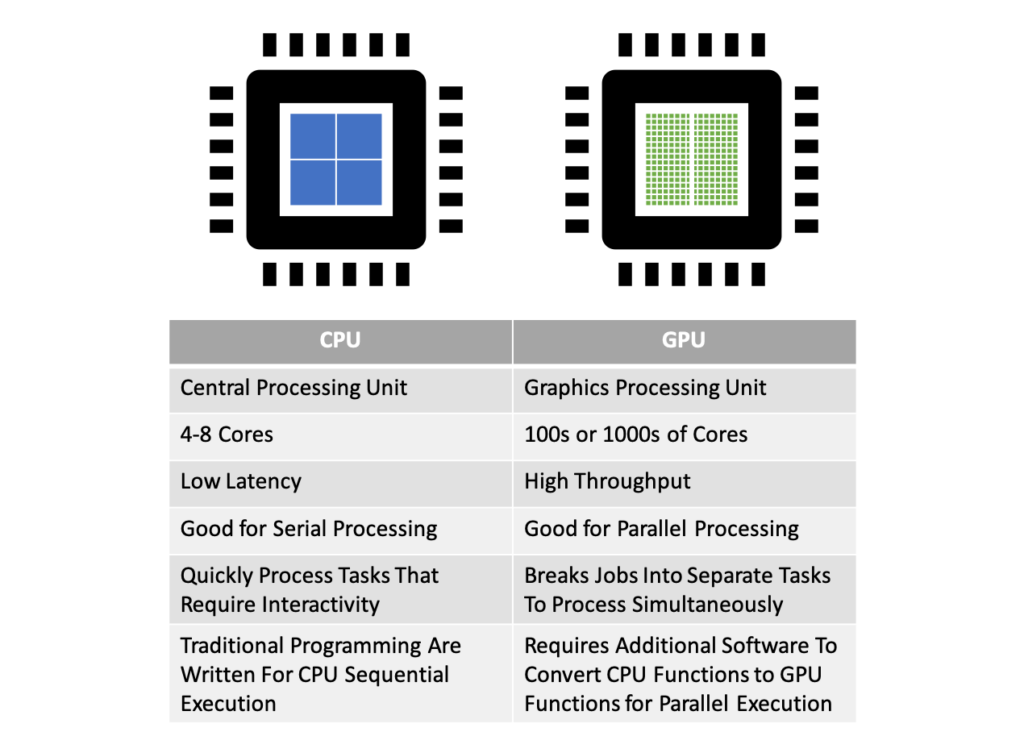
\includegraphics[width=0.8\linewidth,height=\textheight,keepaspectratio]{cpu-gpu-architecture-comparison.png}
  \caption{Comparação simplificada entre arquitetura de CPU e GPU. Fonte:
    \textcite{layerstack2023cpugpu}.}\label{fig:cpu-gpu-contrast}
\end{figure}

A Figura\textasciitilde{}\ref{fig:cpu-gpu-detail} mostra esse contraste
na divisão da área do chip. Em uma CPU típica, poucos núcleos complexos
dividem espaço com grandes caches e lógica de controle. Em uma GPU, o
desenho é o inverso: a maior parte da área é dedicada a conjuntos de
núcleos de processamento paralelos (por exemplo, \emph{CUDA cores} em
GPUs NVIDIA ou \emph{stream processors} em GPUs AMD) e à memória de alta
largura de banda. O controle é mais simples, mas o número de operações
por segundo é muito maior quando o problema é bem mapeado para esse tipo
de arquitetura \autocite{paz2011gpucpuimage}.

\begin{figure}
  \centering
  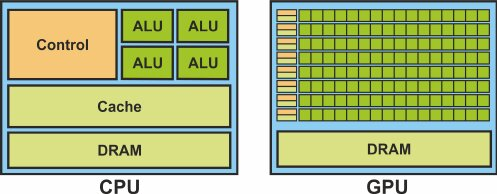
\includegraphics[width=0.8\linewidth,height=\textheight,keepaspectratio]{cpu-gpu-silicon-allocation.png}
  \caption{Alocação de silício em CPU e GPU. Adaptado de
    \textcite{paz2011gpucpuimage}.}\label{fig:cpu-gpu-detail}
\end{figure}

A Figura\textasciitilde{}\ref{fig:gpu-internal} resume como esses
recursos aparecem na organização interna de uma GPU moderna. A memória
global (DRAM) oferece grande largura de banda, mas latência alta; cada
\emph{streaming multiprocessor} (SM) possui memórias compartilhadas
menores e registradores, usados pelas threads de um mesmo bloco. As
threads são agrupadas em \emph{warps} (tipicamente 32 threads nas GPUs
NVIDIA) que executam a mesma instrução ao mesmo tempo, seguindo o modelo
SIMT \autocite{shah2023gpuarchitectureimage}. Quando as threads de um
warp seguem caminhos de controle diferentes ou acessam a memória de
forma muito irregular, parte dessa paralelização é perdida; quando o
acesso é organizado e o fluxo de controle é parecido, o ganho de
desempenho é grande.

\begin{figure}
  \centering
  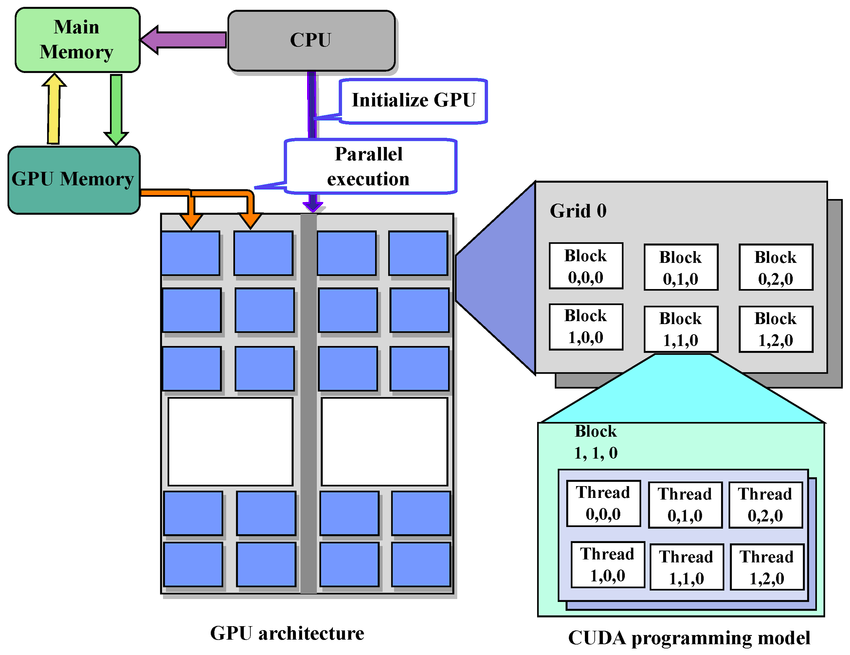
\includegraphics[width=0.8\linewidth,height=\textheight,keepaspectratio]{gpu-internal-architecture.png}
  \caption{Organização interna de GPU moderna e modelo de programação
    CUDA. Adaptado de
    \textcite{shah2023gpuarchitectureimage}.}\label{fig:gpu-internal}
\end{figure}

Essas três figuras servem como pano de fundo para as decisões de projeto
dos kernels CUDA apresentados no Capítulo 3: explorar paralelismo em
dados (tipo 1) mapeando threads para indivíduos ou movimentos \(2\)-opt,
evitar ao máximo divergência dentro de um mesmo warp e organizar as
leituras e gravações de memória global para aproveitar melhor a largura
de banda disponível.

É fundamental distinguir, portanto, três níveis de paralelismo que
aparecem neste trabalho. No nível da máquina, a CPU é tratada como uma
arquitetura MIMD: diferentes núcleos podem executar tarefas distintas ou
\emph{threads} independentes. Dentro de cada núcleo, porém, a CPU pode
explorar SIMD por meio de instruções vetoriais, o que acelera trechos
específicos do cálculo de custos e de manipulação de vetores. Já a GPU,
no contexto de CUDA, é programada no modelo SIMT: o programador escreve
milhares de \emph{threads} lógicas, mas o hardware as executa em grupos
(\emph{warps}) que avançam de forma coordenada enquanto compartilham o
mesmo fluxo de instruções. Quando há divergência de controle dentro de
um \emph{warp}, os caminhos precisam ser serializados temporariamente,
reduzindo a eficiência. Essa distinção explica por que a CPU pode ser
descrita, sem contradição, como MIMD com extensões SIMD, enquanto a GPU
é mais adequadamente descrita como SIMT.

\section{Comparação estatística de algoritmos de otimização}\label{sec-27-comparacao-estatistica}

Meta-heurísticas estocásticas, como GAs e algoritmos meméticos, produzem
resultados que variam de execução para execução devido ao uso de
aleatoriedade em diversos pontos (inicialização, seleção, mutação, entre
outros). Por esse motivo, a comparação de algoritmos de otimização não
pode se basear em uma única execução por instância, tampouco apenas em
médias simples sem análise de variabilidade. A literatura de comparação
de algoritmos enfatiza a importância de utilizar múltiplas instâncias de
teste, múltiplas repetições por combinação algoritmo--instância e
métricas que considerem tanto qualidade da solução quanto tempo de
execução \autocite{demsar2006statistical}.

\textcite{demsar2006statistical} discute procedimentos estatísticos
apropriados para comparar algoritmos em vários problemas, recomendando o
uso de testes de hipótese pareados (como o teste \emph{t-pareado} ou o
teste de Wilcoxon) quando se deseja comparar dois algoritmos em uma
coleção de instâncias, e testes baseados em rankings, como o teste de
Friedman seguido de pós-testes de Nemenyi, quando mais de dois
algoritmos são avaliados simultaneamente. Medidas de tamanho de efeito,
como o \emph{d} de Cohen, complementam a análise ao quantificar a
magnitude prática das diferenças observadas.

Neste trabalho, esses princípios gerais orientam o desenho experimental
e a análise dos resultados apresentados nos capítulos seguintes,
garantindo que as comparações entre variantes em CPU e GPU sejam
realizadas de forma estatisticamente fundamentada. De maneira mais
concreta, para cada combinação algoritmo--instância (4 algoritmos vs 38
instâncias), são executadas múltiplas repetições independentes,
registrando-se, no mínimo, medidas de qualidade da solução (custo final
ou \emph{gap} em relação ao melhor valor conhecido) e de tempo de
execução.

\subsection{Comparações pareadas}\label{sec-271-comparacoes-pareadas}

Para comparações \textbf{par a par} entre duas variantes (por exemplo,
versão puramente em CPU versus uma versão em GPU) ao longo de várias
instâncias, adota-se
uma rotina em duas etapas: (i) verificação de normalidade das
distribuições de interesse por meio do teste de Shapiro--Wilk
\autocite{shapiro1965analysis} e (ii) aplicação de um teste pareado
apropriado. Quando a hipótese de normalidade é considerada aceitável,
utiliza-se o teste \emph{t-pareado} de Student
\autocite{student1908probable}; caso contrário, recorre-se ao teste não
paramétrico de Wilcoxon para amostras pareadas
\autocite{wilcoxon1945individual}. Em ambos os casos, medidas de tamanho
de efeito, como o \emph{d} de Cohen \autocite{cohen1988statistical}, são
utilizadas para qualificar a relevância prática das diferenças
detectadas. Valores típicos de \emph{d} de Cohen são interpretados como:
\(|d| < 0.2\) (efeito negligenciável), \(0.2 \le |d| < 0.5\) (efeito
pequeno), \(0.5 \le |d| < 0.8\) (efeito médio), e \(|d| \ge 0.8\)
(efeito grande). Estas comparações seguem as diretrizes de testes de
``Statistical Comparisons of Classifiers over Multiple Data Sets''
\autocite{demsar2006statistical}, e as fórmulas são de fácil
implementação utilizando bibliotecas em \texttt{python}.

\subsection{Comparações múltiplas}\label{sec-272-comparacoes-multiplas}

Quando três ou mais algoritmos são comparados simultaneamente em um
conjunto de instâncias (como ocorre com as quatro variantes
variantes de estrutura algorítmica comum, descritas na \hyperref[obs-envelope-comparacao]{Seção 3.2}), emprega-se o teste de Friedman \autocite{friedman1937use}
sobre os rankings médios dos algoritmos em cada problema, seguido de
pós-testes de Nemenyi \autocite{nemenyi1963distribution} quando
apropriado, conforme recomendado por \textcite{demsar2006statistical}.
Esse procedimento permite identificar, com controle de erro tipo I,
quais pares de algoritmos apresentam diferenças estatisticamente
significativas em termos de desempenho médio. O teste de Friedman
verifica a hipótese nula de que todos os algoritmos têm desempenho
equivalente, enquanto o pós-teste de Nemenyi ajusta os valores-p para
múltiplas comparações, reduzindo o risco de falsos positivos.

Os detalhes específicos de parametrização desses testes, bem como o
conjunto exato de métricas analisadas (tempo, qualidade, ganho de
performance, entre outras), são apresentados no
\hyperref[cap3-materiais-metodos]{Capítulo 3} ao descrever o protocolo
experimental, e retomados no \hyperref[cap4-resultados]{Capítulo 4} ao
discutir os resultados obtidos.

